\documentclass[a4paper,12pt,twoside]{report}

\usepackage[french]{babel}  % Pour le français
\usepackage[utf8]{inputenc} % Pour taper les caractères accentués

\usepackage{amsmath}  % Ces trois paquets donnent accès à 
\usepackage{amsfonts} % des symboles et formulations
\usepackage{amstext}  % mathématiques
\usepackage{hyperref} % Permet de faire automatiquement des liens dans les
                      % documents
\usepackage{graphicx} % Permet d'insérer des images
\DeclareGraphicsExtensions{.png} % Mettre ici la liste des extensions des
                                 % fichiers images

% On peut choisir la police en utilisant un paquet 
%\usepackage{newcent}
\usepackage{lmodern}
%\usepackage{cmbright} % Computer Modern Bright

% Une des nombreuses manière de modifier les marges par défaut
\usepackage{geometry}
\geometry{vmargin=2cm,hmargin=2.5cm,nohead}

% On peut redéfinir certaines longueurs, par exemple l'espacement entre les
% paragraphes:
\setlength{\parskip}{0.25cm}

% Quelques définitions 
\def \rr {{\mathbb R}} % L'ensemble R
\def \cc {{\mathbb C}} % L'ensemble C
\def \nn {{\mathbb N}} % L'ensemble N
\def \zz {{\mathbb Z}} % L'ensemble Z

% Les informations de la page de titre (page de titre séparée pour un 'report').
\title{Mon premier rapport en \LaTeX}
\author{
  Moi Même\thanks{\href{mailto:yves.coudiere@u-bordeaux.fr}{\tt yves.coudiere@u-bordeaux.fr}}
  \and
  Qq'un d'autre\thanks{Bla bla}
}
% \thanks: permet de mettre une note de bas de page pour l'auteur
% \href: insère un lien, ici vers l'application 'mailto'
% \tt: police monospace
\date{\today} % \today pour la date courante 

\begin{document}

\maketitle % Page de titre automatique à partir des infos ci-dessus

% La commande cleardoublepage est utilisée pour s'assurer que la page suivante
% est une page de droite lorque l'on imprime recto-verso.
\cleardoublepage
\tableofcontents % Table des matière automatique à partir des chapitres,
                 % sections, etc du document

\cleardoublepage
\chapter{Une première section, par exemple une introduction}

On peut facilement insérer des équations dans le texte, par exemple
$3x^2+5 = 0$, où encore des égalités intégrales, comme
$\int_0^1 \frac{1}{1+x^2} dx = \frac{\pi}{4}$.

% les espacements entre paragraphes, indentation, etc sont automatiques.

On peut aussi mettre des équations hors texte, et les numéroter automatiquement:
\begin{equation}
  \label{eq:exemple}
  y'(t) = f(t,y(t)).
\end{equation}
Il devient alors très simple de faire référence à une équation, grâce à son {\tt
  label}. Ici on peut discuter de l'équation différentielle~\eqref{eq:exemple}.

\cleardoublepage
\chapter{Une deuxième section}

\section{Sous-section modélisation}

Pour faire une référence bibliographique, le principe est le même. Par exemple,
on trouve des résultats classiques de l'analyse et de l'analyse numérique des
méthodes de résolution des équations différentielles dans le  livre de
M. Crouzeix et A.L. Mignot \cite{crouzeixmignot}.

\section{Ce qu'on cherche à faire}

Un autre référence bibliographique, vers un article \cite{rush_larsen.1978}
plutôt qu'un livre. Dans ce document, les références sont listées dans un
fichier spécial d'extension {\tt .bib}, dans notre cas, le fichier {\tt
  refs.bib}.
\begin{figure}[htpb!]
  \centering
  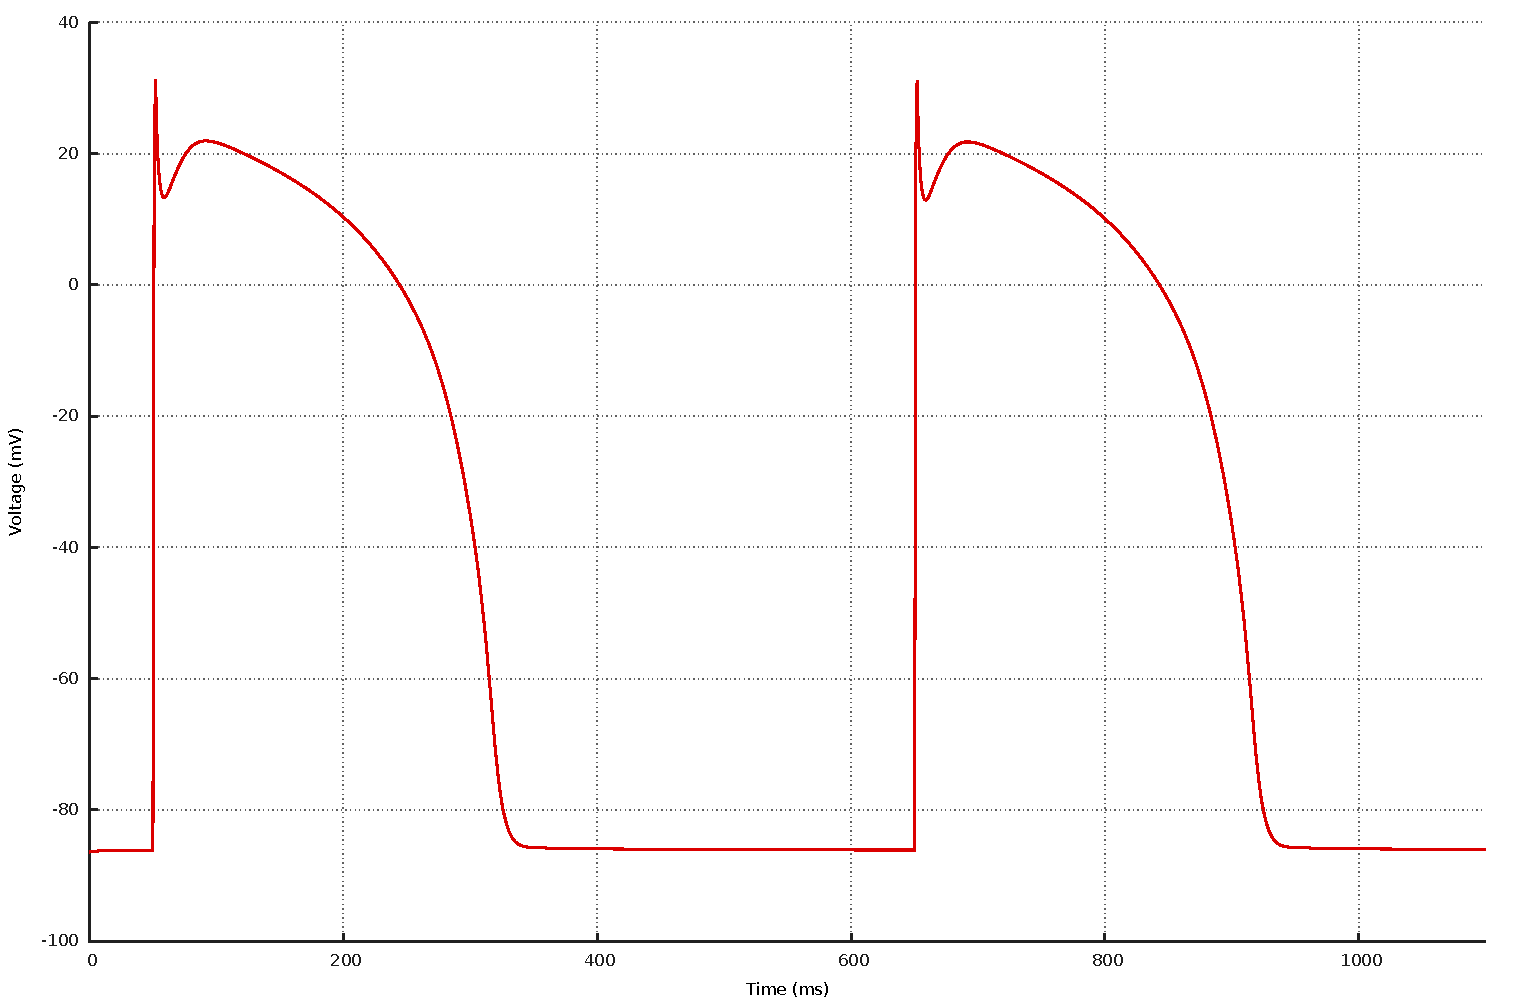
\includegraphics[width=0.8\linewidth]{V_tnnp.pdf}
  \caption{Exemple de figure montrant une image, format pdf.}
  \label{fig:exemple}
\end{figure}

Bien sur, on référence les figures comme les équations, grâce à leurs {\tt
  label}. La figure~\ref{fig:exemple} montre deux potentiels d'action cardiaques
consécutifs.

\cleardoublepage
\bibliographystyle{plain}
\bibliography{refs}

\end{document}

